\documentclass[12pt,letterpaper]{article}
\usepackage{fullpage}
\usepackage[top=2cm, bottom=4.5cm, left=2.5cm, right=2.5cm]{geometry}
\usepackage{amsmath,amsthm,amsfonts,amssymb,amscd}
\usepackage{lastpage}
\usepackage{enumerate}
\usepackage{fancyhdr}
\usepackage{mathrsfs}
\usepackage{xcolor}
\usepackage{graphicx}
\usepackage{listings}
\usepackage{hyperref}

\hypersetup{%
  colorlinks=true,
  linkcolor=blue,
  linkbordercolor={0 0 1}
}
 
\renewcommand\lstlistingname{Algorithm}
\renewcommand\lstlistlistingname{Algorithms}
\def\lstlistingautorefname{Alg.}

\lstdefinestyle{Python}{
    language        = Python,
    frame           = lines, 
    basicstyle      = \footnotesize,
    keywordstyle    = \color{blue},
    stringstyle     = \color{green},
    commentstyle    = \color{red}\ttfamily
}

\setlength{\parindent}{0.0in}
\setlength{\parskip}{0.05in}
\begin{document}





Sunny Lee\\
Foundations of Applied Math\\
 HW \#7 Stability of Equilibria of Systems of Differential Equations (From 12.1) and Review.\\
 Please understand that you have been taught everything you need to know to do this HW except for problem 5. I will cover how to do problem 5 on Monday.\\
 Due Friday, Oct. 30 by 7 am
 
\textbf{Reminder} You need to turn in a .zipped folder that contains your .tex file, your image files, your python files, your Excel file(s), and the tex file must compile.
Rename the .tex file: HW7$\_$YourLastName.tex and call the folder which you will compress: HW7$\_$YourLastName


\begin{enumerate}
\item  (Review) Do the root finding classwork Problem \#2 from Tuesday, Oct. 20 using Excel. Please include your Excel file in your HW folder.\\
\emph{Solution.}
Using Newton's method, we find the first positive root to be about $2.00370042$, which 
is exactly the same number we got using python: \\
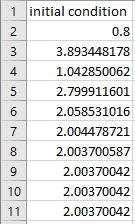
\includegraphics{number1.png}\\
number1.xlsx is included. 

\item  (Review) Given the following system:
\begin{eqnarray*}
\frac{dx}{dt} &=&-x+y\\ \\
\frac{dy}{dt}&=&-x-y\\
\end{eqnarray*}

\begin{enumerate}[a)]
\item Verify that $x=e^{-t}\sin(t)$ and $y=e^{-t}\cos(t)$ solve this differential equation system.\\
For our first equation $\frac{dx}{dt}$: 
\begin{eqnarray}
  \frac{d}{dt}(e^{-t}\sin(t)) &\stackrel{?}{=}& -e^{-t}\sin(t) + e^{-t}\cos(t)\\
  - e^{-t}\sin(t) + e^{-t}\cos(t) &\stackrel{}{=}& -e^{-t}\sin(t) + e^{-t}\cos(t)\\
\end{eqnarray}

So we have found our $x$ and $y$ solve $\frac{dx}{dt}$. For our $\frac{dy}{dt}$: 
\begin{eqnarray}
  \frac{d}{dt}(e^{-t}\cos(t)) &\stackrel{?}{=}& -e^{-t}\sin(t) - e^{-t}\cos(t)\\
  -e^{-t}\sin(t) - e^{-t}\cos(t) &\stackrel{}{=}& -e^{-t}\sin(t) - e^{-t}\cos(t)
\end{eqnarray}
and thus, we find that both of our functions are solutions to our system of 
differential equations.

\item  Find the equilibrium solution(s).\\
For $\frac{dx}{dt}$: 
\begin{eqnarray*}
  -x+y &=& 0\\
  y &=& x
\end{eqnarray*}
Plugging this into our second equation: 
\begin{eqnarray*}
  -x - y &=& 0\\ 
  -y - y &=& 0\\
  -2y &=& 0\\
  y &=& 0
\end{eqnarray*}
Plugging $y=0$ into our original equation: 
\begin{eqnarray*}
  0 &=& x
\end{eqnarray*}
So we find that we have one equilibrium solution at $(0, 0)$


\item  Take the system of  exact solutions in part a, square both sides and add them together. What equation do you get? This should be a form that you recognize. Name the curve and any properties about this curve.
\\
Using the two solutions in part a: 
\begin{eqnarray*}
  x^2 = e^{-2t}\sin^{2}(t)\\
  y^2 = e^{-2t}\cos^{2}(t)\\
  x^2 + y^2 = e^{-2t}(\cos^2(t) + \sin^2(t))\\
  x^2 + y^2 = e^{-2t}
\end{eqnarray*}
This is the equation of a circle with radius $\sqrt{e^{-2t}} = \pm e^{-t}$. So, when 
$t$ is constant, we find that it is a circle with radius $\sqrt{e^{-t}}$. As $t \rightarrow \infty$, 


\item  Using python, plot $x$ vs $t$ and $y$ vs $t$ on the same graph. Include your code and paste your graph here.\\
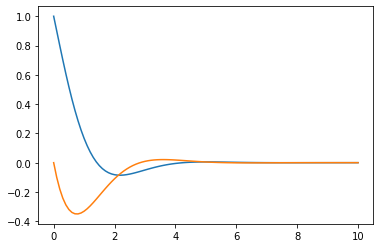
\includegraphics{yxvst.png}\\
number2.py is included in the zip.

\item Using python plot $y$ vs $x$ on another graph. Include your code and paste your graph here.\\
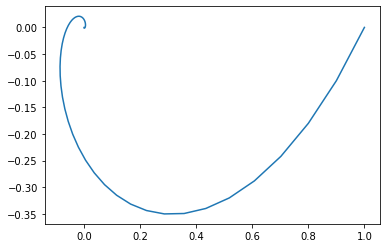
\includegraphics{yvsx.png}\\
number2e.py is included in the zip.
\end{enumerate}



\newpage
\item   (Review) Consider
\begin{eqnarray*}
\frac{dx}{dt} &=& 0.04x-.0005xy\\
\frac{dy}{dt} &=&-0.2y+.00049xy\\
\end{eqnarray*}

\begin{enumerate}[a)]
\item Find $\frac{dy}{dx}$. This is just algebra and you don't have much simplication to do.
\\ \emph{Solution.}\\

\begin{eqnarray*}
  \frac{dy}{dx} &=& \frac{dy}{dt} \frac{dt}{dx}\\
  \frac{dy}{dt} \frac{dt}{dx} &=& \frac{-0.2y + .00049xy}{0.04x - .0005xy}\\
  \frac{dy}{dx} &=& \frac{-0.2y + .00049xy}{0.04x - .0005xy}
\end{eqnarray*}


\item Use Euler's Method on your differential equation that you found in part a, to approximate the value of $y$ in the table below (show your work below the table- your are doing this calculation by hand):

\begin{eqnarray*}
  y_1 &=& y_0 + \Delta x \frac{dy}{dx}\\
  y_1 &=& 10 + 25(\frac{-0.2(10) + .00049(55)(10)}{0.04(55) - .0005(55)(10)})\\
  y_1 &=& - 12.474025974
\end{eqnarray*}

\begin{eqnarray*}
  y_2 &=& y_1 + \Delta x \frac{dy}{dx}\\
  y_2 &=& - 12.474025974 + 25(\frac{-0.2(- 12.474025974) + .00049(80)(- 12.474025974)}{0.04(80) - .0005(80)(- 12.474025974)})\\
  y_2 &=& 1.08264139484
\end{eqnarray*}

\begin{center}
\begin{tabular}{| c| c |c| }\hline
$n$ & $x$& $y$ \\ \hline
0 &55 & 10  \\ \hline 
1 &80 &  - 12.474025974\\ \hline
2 &105 & 1.08264139484 \\ \hline
\end{tabular}
\end{center}


\item Which population seems to be changing at a faster rate: $x$ or $y$? Why?\\
 $x$ seems to be changing at a faster rate, as our $\Delta x$ value is greater than 
 $y_1 - y_0$ and $y_2 - y_1$. 

\item  In part b, the $y-$values were estimated using $h=\Delta x=$ what value? Explain.
\\
Our $\Delta x$ value was $25$, as the difference between $x$ values was consistantly 25. 

 \item Describe how decreasing the value of $\Delta x$ would affect the accuracy of Euler's Method.
 \\
 Decreasing the value of $\Delta x$ would improve the accuracy, as we are taking
 smaller steps when approximating our new $y$ values, so our change in $y$ 
 is more accurate at each step. 
 
\item Write a python program that uses Euler's Method to solve the differential equation that you found as your answer to part a over the same $x$ values that you are given in part b.  Have your output only be three $(x,y)$ pairs. I don't want the graph. You should get the same values that you got by hand.  You already know the first $ (x,y)$ pair: 55 and 10 (given).
Include your python code and output.
\\
From our Euler's method output, we find: \\
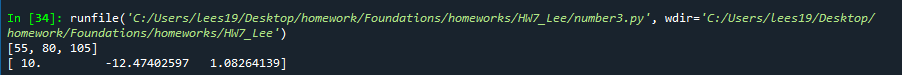
\includegraphics[scale = .7]{number3f.png}\\
Which were exactly the same values we got when we did the calculations by hand. 
The code is in number3.py. 

\end{enumerate}
\newpage
\item  (Review) Given that the exact solution to the initial value problem  $y^{\prime}=y, y(0)=1$ is the function,  $y=e^{t}$  write a program that will compute the average percent error for a given $h$.   Percent error is defined as:
$$\frac {| \mbox{Theoretical} - \mbox{Approximate} |}{|\mbox{Theoretical} |} \times 100\% $$


When you are done, fill in this table using your python program:

\begin{tabular}{| l| l|} \hline
$h$ & Average Percent Error \\  \hline
1   &  26.424112\%                     \\ \hline
0.5 &  13.123763\%                     \\ \hline
.25 &  6.451519\%                    \\ \hline
.125 & 3.182229\% \\ \hline
\end{tabular}


 
 
Suggestions:
 
 
\begin{enumerate}[a)]

\item Include a function in your code for the exact solution. Recall from a Blackboard post that $e^{5}$, for example, can be coded as 
{\tt np.exp(5)} after you have imported numpy as np.)

\item  At each time step output the percent error. Please note that  to calculate absolute value in Python use the {\tt abs()} function.  \emph{Hint} Because your  final task is to compute the average percent error for a given $h$, (see above part a)  I would suggest that you keep the percent errors at each time step in an array.


\item As mentioned above your program  needs to compute the average percent error for each $h$.  Have your program output a line that says ``For $h$ = ''   the average percent error ='' so that you can fill in the table and so that I can follow your code output easily.


\item I would advise you to use the {\tt sum} function in python to compute the sum of the elements of an array if you store your errors for each $h$ in an array. You need a sum since you are computing an average (sums go in the numerator). Here's an example of how to use the sum is the following. Suppose you have an array called 
{\tt Q} that has 2 elements: {\tt Q[0] = 1 } and {\tt Q[1]=2}. then {\tt sum(Q)} =3.

\item You will know if you are doing this problem correct if you obtain 3\% is the average percent error when $h=0.125$ (that's the last row answer in the table above.

\end{enumerate}

\emph{Solution}\\
number4.py is included in the zip file.

\newpage
\item Section 12.1)  I will cover on Monday
 \begin{eqnarray*}
 \frac{dx}{dt} &=& 4x-xy-2x^2\\
 \frac{dy}{dt} &=& 2y-xy-3y^2
\end{eqnarray*} 
\begin{enumerate}[a)]
\item Explain the physical significance of the term $2x^2$ and the -$xy$ term in the first equation.
\\\emph{Solution.} \\
The $2x^2$ term means there is intracompetition going on within the $x$ population. If we 
assume there are no interactions between the $x$ and $y$ populations (y = 0), then we 
also see that this term along with the $4x$ term limits the maximum population of the 
$x$ population. The $-xy$ term shows that there is also competition going on between 
the $x$ population and the $y$ population where the $x$ population goes down 
when there are interactions between the $x$ and $y$ populations.

\item Sketch the phase portrait of this problem. Show your work: x-nullclines, y-nullclines, rest points, arrows.
\\\emph{Solution.} \\
x-nullcline: y = -2x+4\\
y-nullcline: y = -$\frac{x}{3} + \frac{2}{3}$\\
Rest points: $(0, 0)$, $(0, 2/3)$, $(2, 0)$\\
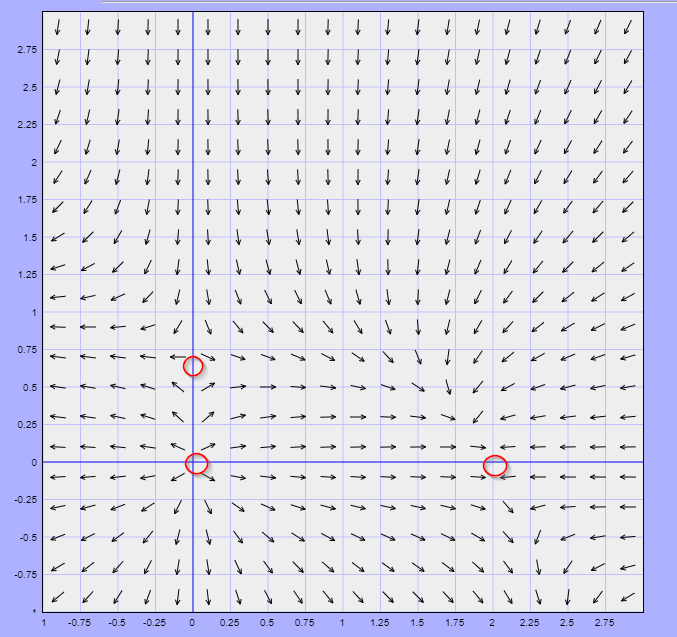
\includegraphics[scale = .5]{number5b.png}\\

\item Using your phase plane portrait, determine the stability of each of the fixed points.
\\\emph{Solution.}\\
Using the phase plane, we find that all three of our rest points are unstable, as 
every rest point has arrows pointing out from the rest point.

\item  This system is modeling two different populations with time. Is it modeling a  predator-prey relationship or a competition model? Explain.
\\ \emph{Solution}\\
This is a competition model, as the interactions between populations (and between themselves)
only hurts the total population of $x$ and $y$. 

\item What is the long-term behavior of the physical system? Is there a species that always wins? Does it
depend on the initial population levels? Explain how this could make sense.
\\ \emph{Solution.}\\
Long term, it seems that the $x$ population always wins. No matter where we put our 
initial solutions, they all seem to converge to our rest point $(2, 0)$, meaning 
no matter which initial condition we pick(in the first quadrant), in the long term, the $y$ population 
always goes to zero and our $x$ population goes to $2$. 

\item Use the method from \#6 of HW 6 with $h=0.1$ to approximate the solution to this differential equation system three times with three sets of initial conditions: choose initial conditions to be in each of the three quadrant 1 regions that you found above.  Include either your .py file. And include the four plots here, labelled with their corresponding initial conditions. Verify if your graphs can help explain the long term behavior.
\\\emph{Solution.}\\
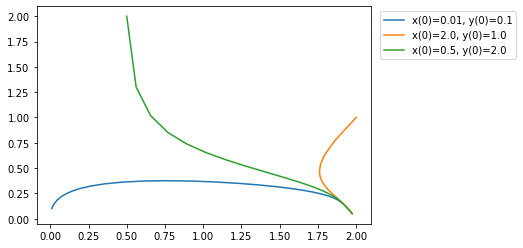
\includegraphics[scale = .8]{number5f.png}\\
All three initial conditions converge to $(2, 0)$ which we saw in part $e$. Since we 
seem to be getting $(2, 0)$ for all three initial condtiions in our three regions, we 
see this is a good way to verify the long term behavior of our system of differential 
equations.
\end{enumerate}

\end{enumerate}
\end{document}